\section{Communication View}

The autonomous cars need to gather information on their environment. This can only be done through a multiple exchanges between the vehicles but also with a centralized station. Therefore, the vehicles must be able to communicate  with other systems. In this part, we will study different protocols used for communication.

\subsection{Automotive software in connected vehicles}

In 2020, we estimate that 75\% of the cars will have the capacity to connect to the Internet, with a connectivity with connected object as smartphones.The article \cite{connectivity_car}, written by Hrvoje Vdovic from the Faculty of Electrical Engineering and Computing, University of Zagreb, Zagreb, Croatia, makes a review of the different information and communication technology (ICT) for connected and autonomous electric vehicle (CAEV).

The paper describes the softwarized architecture with a high level point of view. The system is composed by Electronic Control Units (ECUs) which is responsible for vehicle’s functions. The networking of ECUs is made with automotive bus system divided in 4 communication group: event-triggered bus systems, time-triggered bus systems, subnetworks and multimedia bus systems. The Control Area Network (CAN) is an event-triggered bus mainly used for real-time soft.

With connected vehicles, we can see 4 mainly types of communication:

\begin{itemize}
    \item Vehicle to Vehicle (V2V)
    \item Vehicle to road infrastructure
    \item Vehicle to Internet
    \item Vehicle to smart device
\end{itemize}

The internet communication is achieved either by a Telematics Control Unit, a module with a card SIM permanently installed, or by a modem which allows the use of a personal SIM card or either by a user’s smart device. 4G mobile communication allows communications with Internet and the communication with a smart device by a Bluetooth or Wi-Fi connection.

In the future, the automotive software development tends to aim four different goals: energy and cost efficiency, zero accidents, seamless connectivity and personalization. The paper identifies the main technological trends in automotive software:

\begin{itemize}
    \item Computer architecture centralization (decrease the number of ECUs and undesired interaction)
    \item Standardized communication, Ethernet may replace the current communication buses
    \item Connectivity and cooperation, challenges are the smart device communication and V2V communication
    \item Autonomous functions
\end{itemize}

\subsection{V2I}

Communication with infrastructures offers many new options to manage traffic. We will develop a solution based on V2I communications among others \cite{v2i_management}.

They used a local control station to collect information from the infrastructures or the vehicles to determine a driving state based on vehicles' information and road layout. The station controls the following:
\begin{itemize}
    \item The classification of vehicle within the driving area
    \item Identify stopped vehicle
    \item Inform every vehicle the modification of current speed or if overtaking is possible in straight road
    \item Provide information about road layout in bend stretches
    \item Identify traffic situation of risk
\end{itemize}

Researchers studied  V2I communication in order to manage the traffic flow. They defined two data packages for information exchange (the Reserved field can be used to exchange other information depending on the context): 

\begin{center}
    \begin{figure}[ht!]
        \centering
        
        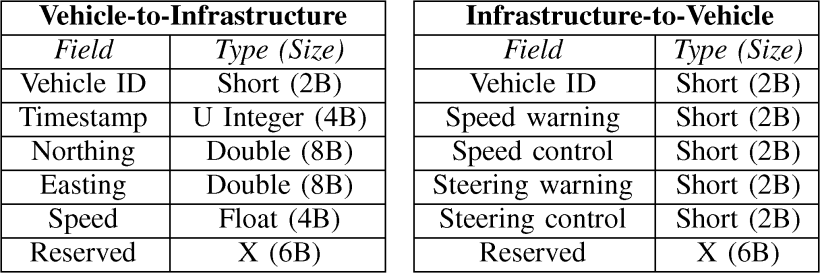
\includegraphics[width=400px, keepaspectratio]{imports/data_package_v2i_communication.png}
        
        \caption{Communications Data Packages}  
        \cite{v2i_management}
    \end{figure}
\end{center}

The communication is achieved by WAVE \cite{v2i_management} communication based on IEEE 8021.11p standard that proposes enhanced distributed channel access (EDCA). EDCA defines four different traffic classes with different priorities:  AC\_VO (Voice Access Category),AC\_VI (Video Access Category, generally unused),  AC\_BE (Best-Effort Access Category) and  AC\_BK (Background Access Category). AC\_VO can only be used by few vehicle and so is kept to special situation as emergency. The challenge is to maintain the delay and packet-loss under a certain limit.
\smallskip

A higher layer mechanism on top of the WAVE stack must be build for critical message dissemination. Unfortunately, the conditions of this applications involve that to maintain the quality of service and real-time application, the number of stations must be less than 40.

\smallskip

In order to handle every kind of situations that can occur, the control station gives the same importance to each car. The car use the collected information they need to make decision. These information are mainly the distance to the vehicle ahead and its velocity. The information is then compared to the references and adapted to their behavior properly. The driving state is also sent by the control station so that the car is aware of the current level of risk.

\smallskip

The driving state \cite{v2i_management} of the car is ranged between -1 and 1 which illustrates the compromise between safety and traffic flow: 0 represent the perfect compromise whereas -1 stands for safe but poor traffic flow and 1 represents the presence of risk of car accident. Therefore the cars try to keep their driving state a little under 0 to ensure the safety of the vehicle.

To check if the driving state was reflecting the real behavior of the car, the researchers tested several scenarios if the car exceeded the recommended velocity. As mentioned in the figure below, the results showed that the driving state was coherent with the situation: when the car exceeded the target velocity, the driving state got closer to 1 and it resulted in a collision.

\begin{center}
    \begin{figure}[ht!]
        \centering
        
        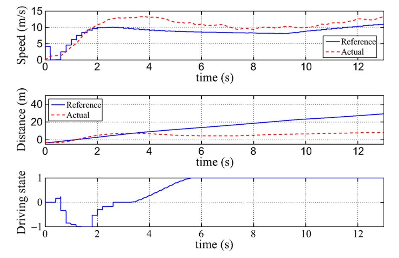
\includegraphics[width=400px, keepaspectratio]{imports/graph_driving_state.png}
        
        \caption{Coherence of the driving state with the situation}  
        \cite{v2i_management}
    \end{figure}
\end{center}




\subsection{oneM2M Standard}


OneM2M was created in 2009 by a group of seven organizations working in the field of standards and industry \cite{alaya_toward_2015}
The main purpose of the oneM2M standards is to unify the different “M2M isolated services” into one norm used by everyone.
\smallskip

A oneM2M system is modeled by four types of nodes: “application dedicated node (ADN), application service node (ASN), middle node (MN), and infrastructure node (IN).” \cite{alaya_toward_2015} An application node is high level whereas an infrastructure node is low level.

oneM2M also aims to solve the problem of interoperability definitively so that those connected object should be able to communicate with another one even if it is a heterogeneous device.
\smallskip

However, oneM2M standard initially does not include semantic data. In other words, data used by oneM2M are not standardized using an ontological model. Ontology is the way to structure data for example adding meta-data in order to specify their semantic. Therefore it was difficult for the applications to understand the meaning of the data exchanged. That was one of the reasons why OM2M was created.


\subsection{OM2M Framework}

OM2M is a framework which aims to make the development of IoT applications easier. It was developed by three researchers of the LAAS-CNRS: Karima Khadir, Thierry Monteil and Samir Medjiah \cite{SicariSabrina2015SOSP}. As the name implies, it respects the oneM2M standard.
\smallskip

This framework proposes that a server should gather the information of each sensor and the data collected from the sensors by the IDE-OM2M.
The OM2M platform has several functionalities:  
\begin{itemize}
    \item Automatic discovery of connected devices
    \item Notification of subscribers to the arrival of new events
    \item Efficient routing 
\end{itemize}
It also uses the HTTP standard in order to exchange data through GET requests for instance.
\smallskip

OM2M has several benefits over other platforms: One of them is syntactic and semantic interoperability. It enables the applications to "understand" the meaning of the information they received from other devices. OM2M added two options to describe the semantic of a resource.
Secondly, this architecture is decentralized because one device can use several OM2M platforms which is not the case for other platforms.
\smallskip

It also has a graphical environment based on Node-RED and it is very intuitive for the user. Nevertheless, several softwares and platforms already developed and used their own framework. The article also listed nine alternative frameworks. Therefore, we can always find a suitable framework which suits to our needs.
\smallskip

The article provides us an example of application: Luminosity control in a building \cite{SicariSabrina2015SOSP}. One OM2M entity is used to collect the information of luminosity in the room. A Semantic Actuactor selects the lamp in the database which consumes the least energy. The lamps are lit until the specified limit is reached.
The article explains in the conclusion that they want to cooperate with NCTU University in order to develop the OM2M framework.